\documentclass[a4paper,10pt]{article}
\usepackage[utf8]{inputenc}
\usepackage{graphicx}
\usepackage{listings}
\usepackage{physics}
\usepackage[margin=1in]{geometry}
\usepackage{subcaption}
\usepackage{float}
\usepackage{hyperref}


\lstset{basicstyle=\footnotesize, breaklines = false}

\date{\today}
\title{FYS-MENA4111 - lab report 4}
\author{Mikael B. Kiste}

\begin{document}
	\maketitle
In this datalab we explored how to view and interpret information about the electronic band structure of our material.
Using some very neat python scripts\footnote{Made by \href{https://www.mn.uio.no/fysikk/english/people/aca/olem/}{Ole Martin}} we can easily get an impression of the shape of the electronic structure of bulk Si as simulated by DFT.
\begin{figure}[H]
	\centering
	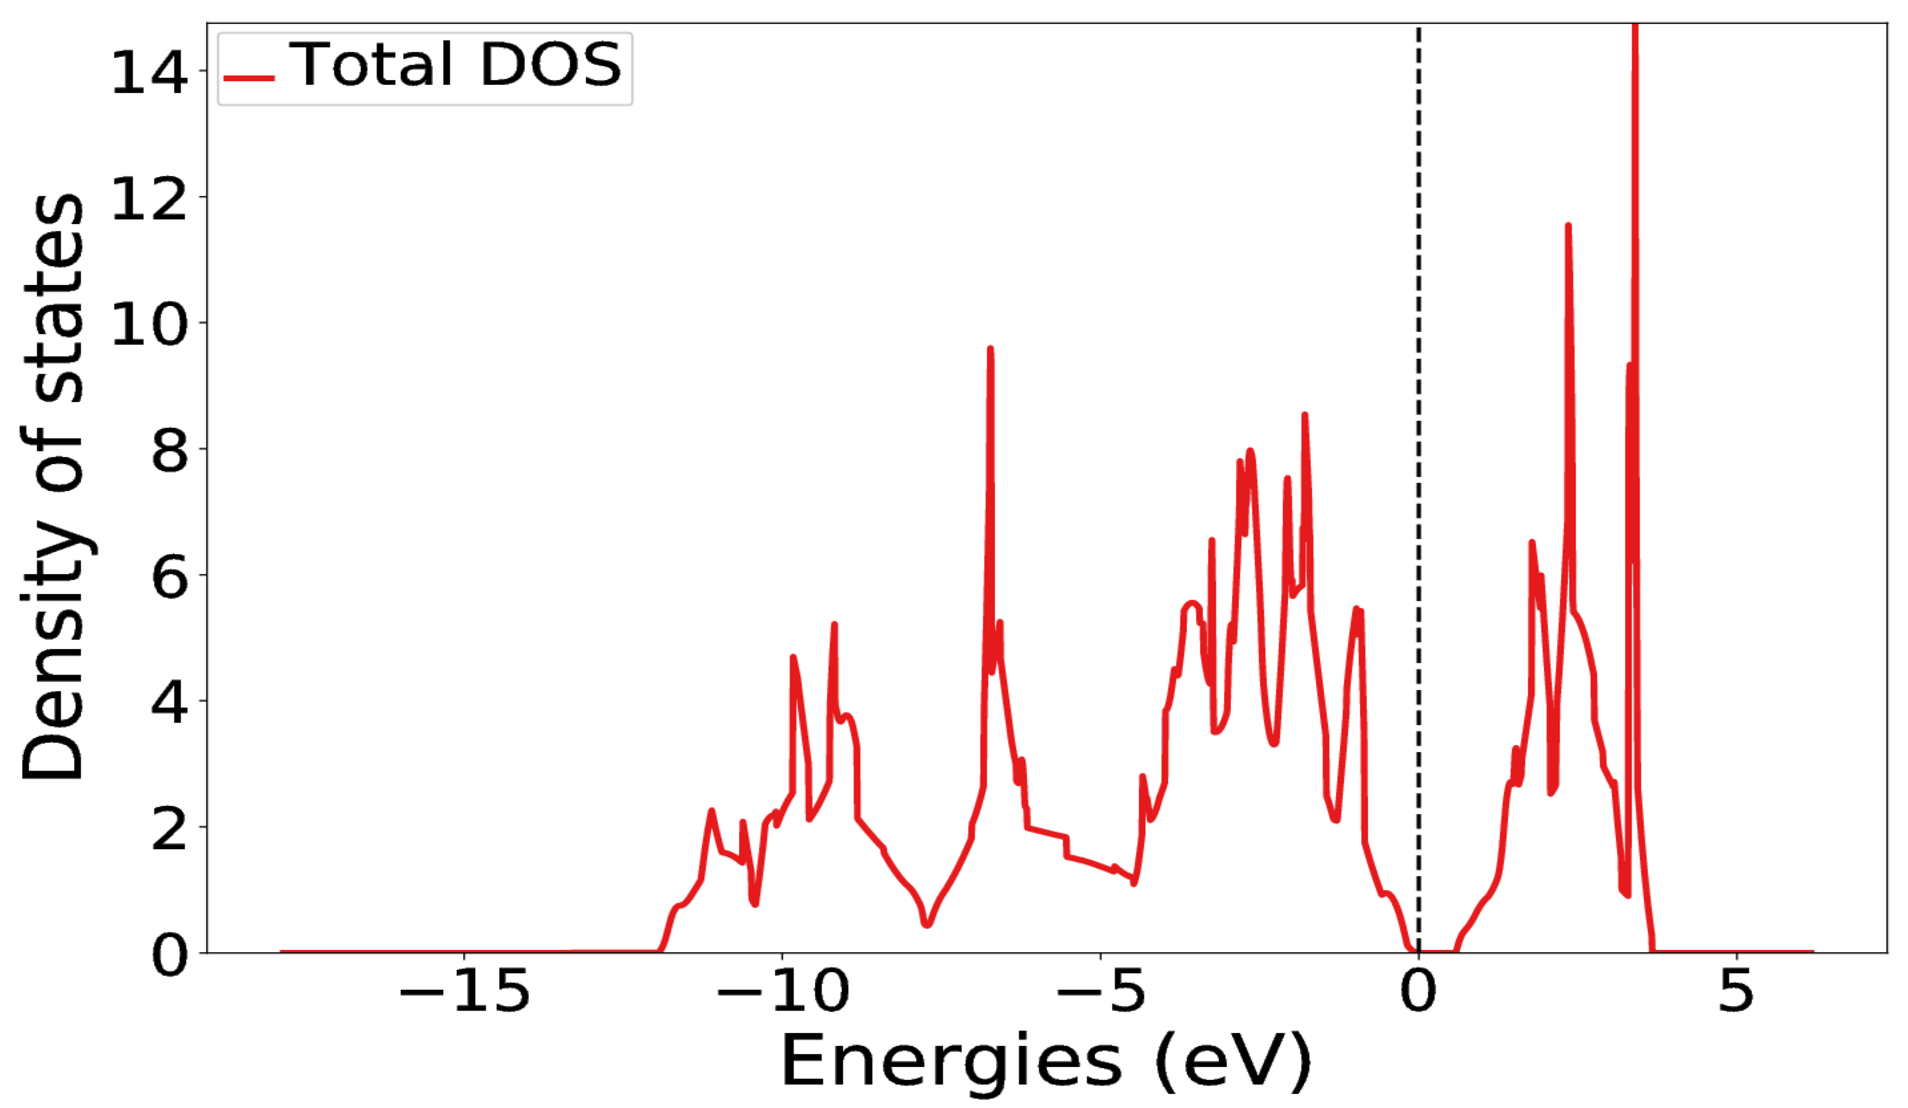
\includegraphics[width=0.7\linewidth]{TDOS}
	\caption{A plot of the DOS as function of energy. One can clearly see the band gap starting from around 0eV}
	\label{fig:tdos}
\end{figure}
A higher value here indicate that there is a high Density of States for that particular energy which in turn, of course, means more electrons capable of existing at that energy inside the material.
The calculated bandgap for Si is 0.5868 eV. This however, does not match very well with the experimental bandgap of 1.2 eV. This is a known weakness of DFT and should always be taken into consideration when evaluation results.

\newpage
We can also get a plot off the so-called projected (or local) Density of States, LDOS.
\begin{figure}[H]
	\centering
	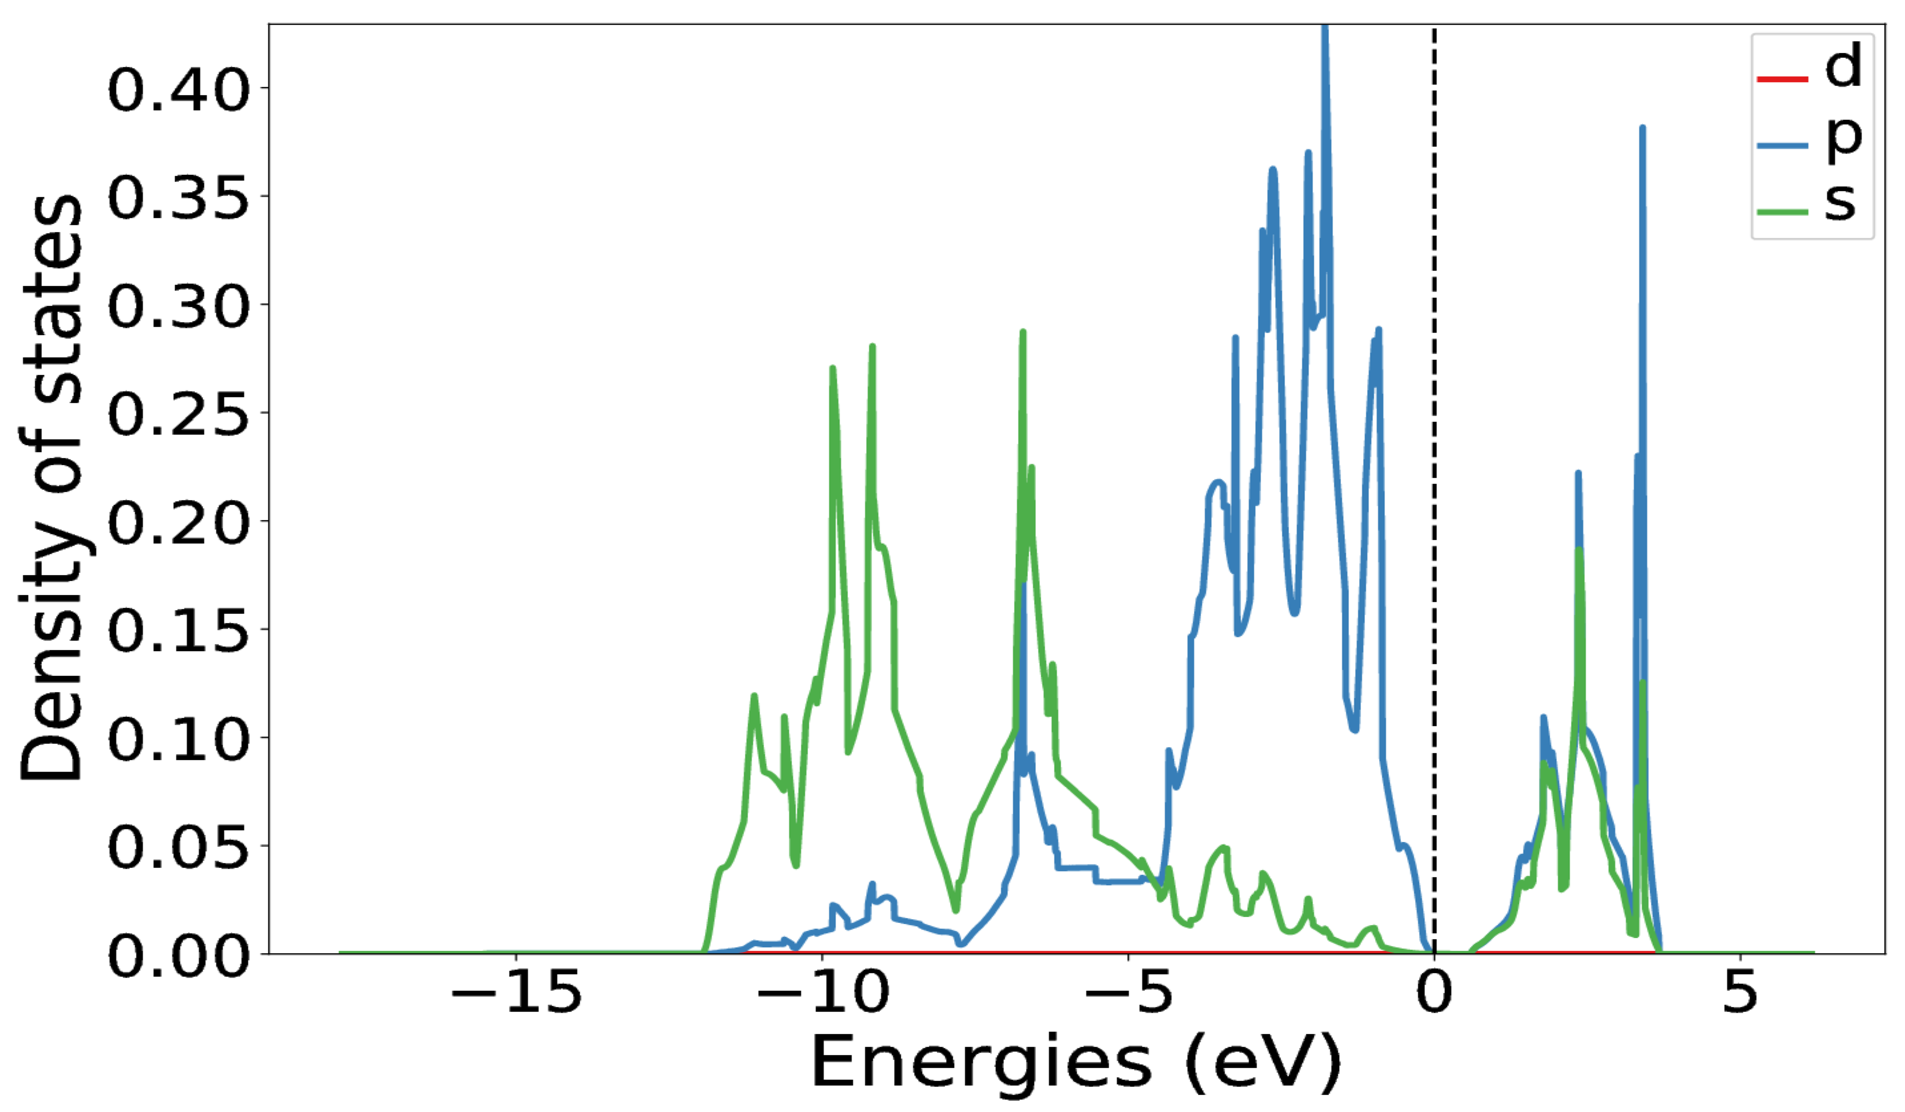
\includegraphics[width=0.7\linewidth]{LDOS1}
	\caption{An LDOS plot of the band structure as a function of energy. There are pretty definitive distinct regions differentiating the preferred locations of the different orbitals}
	\label{fig:ldos1}
\end{figure}
This time we also get explicit information about the orbital quantum number, $\ell$, of the electrons occupying different states (where s, p and d correspond to $\ell=$ 0, 1 and 2 respectively)\\

The Brillouin zone of an FCC lattice is a truncated octahedron
\begin{figure}[H]
	\centering
	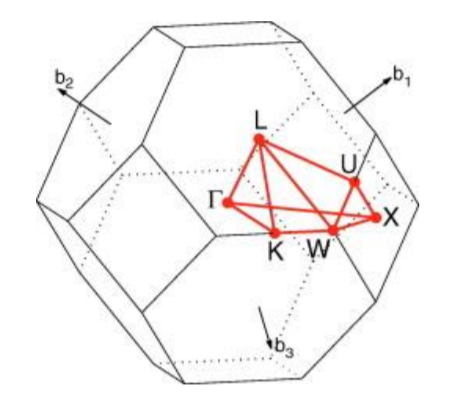
\includegraphics[width=0.7\linewidth]{reciprocal}
	\caption{}
	\label{fig:reciprocal}
\end{figure}
\newpage
The points indicated are points of both high symmetry and interest.
We can actually plot the band structure as a function of moving about from one point to another in reciprocal space. A plot like this is displayed below
\begin{figure}[H]
	\centering
	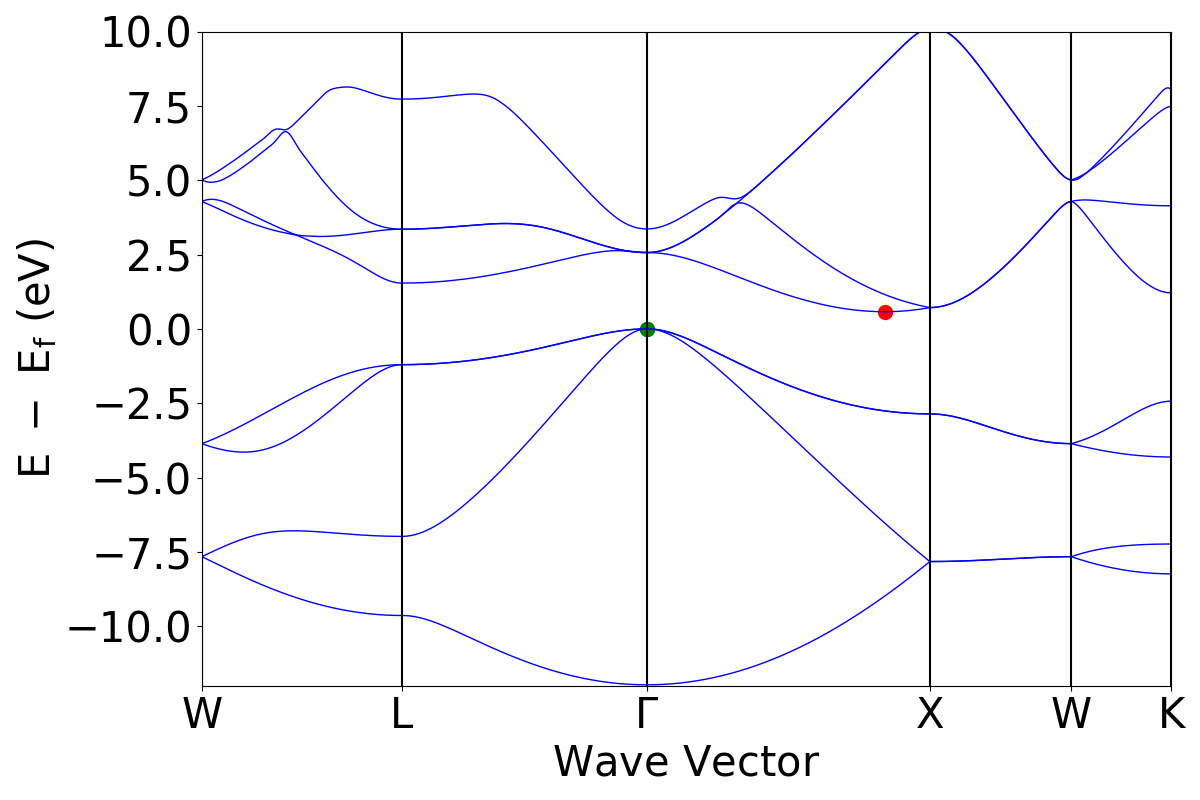
\includegraphics[width=0.7\linewidth]{bandstruct}
	\caption{Band structure of bulk Si between different high symmetry points}
	\label{fig:bandstruct}
\end{figure}
The plot indicates that we have an indirect bandgap with the conduction band state at highest energy is located at the gamma point and the valence band state with the lowest energy is close to X (a BZ side).
Comparing this with the findings of \href{https://www.researchgate.net/publication/270895624_Microscopic_electronic_wave_function_and_interactions_between_quasiparticles_in_empirical_tight-binding_theory}{R. Benchamekh et.al.} we can see that there is a decent correlation between them.
\begin{figure}[H]
	\centering
	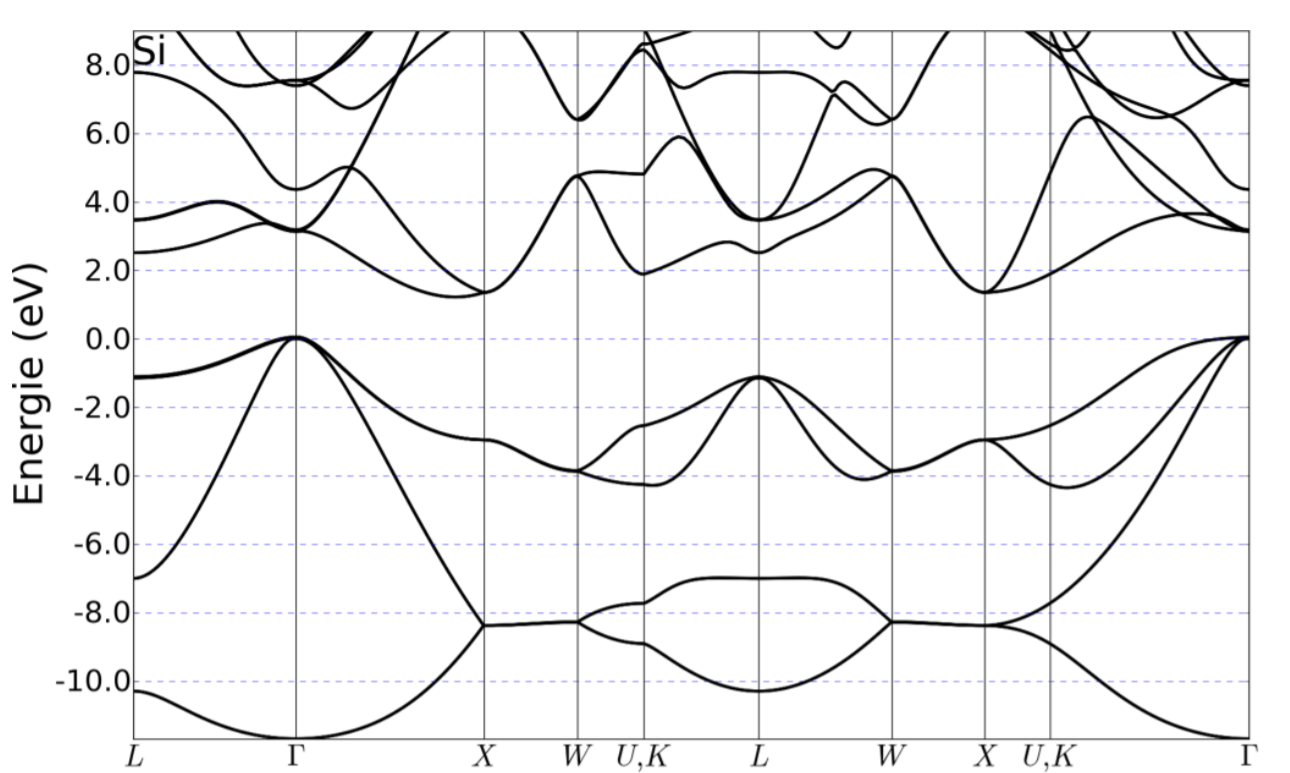
\includegraphics[width=0.7\linewidth]{si_band}
	\caption{}
	\label{fig:siband}
\end{figure}

\end{document}


